\chapter{Lecture 10: Bernoulli random variables and the binomial distribution} \label{lect10}
\section{Bernoulli Random Variables} \label{bernoulli random variable}
A Bernoulli random variable is a random variable (see section \ref{sec8.10}) whose range is a set containing only two values (usually we choose the two values to be $1$ and $0$). In other words, a Bernoulli random variable, $X$, is a function whose domain is $\Omega$ and whose range is $\set{1,0}$. Usually we take $1$ to mean ``success'' and $0$ to mean ``failure.'' So, for any outcome $\omega \in \Omega$ we can have either
\[
X(\omega) = 1 \;\;(\text{success}), \qquad \text{or} \qquad X(\omega) = 0\;\; (\text{failure}).
\]
See section \ref{sec8.1} for a refresher on how we can assign probabilities to the outputs of a random variable. Suppose that we want to assign a probability to the output value $1$ (i.e., a probability of success). Then we are really assigning a probability to the set
\[
\set{X = 1}
\]
Which (according to our definition of this notation in section \ref{sec8.1}) is the set of outcomes from $\Omega$ that are mapped to $1$ by $X$. Since $X$ is a function, it has to map \textit{everything} in its domain to something, so all of the remaining elements in $\Omega$ must be getting mapped to $0$. This means that,
\[
\set{X = 0} \cup \set{X = 1} = \Omega.
\]
It follows that
\[
P\brac{\set{X = 0} \cup \set{X = 1}} = P(\Omega).
\]
We can rewrite the left hand side as
\[
P\brac{\set{X = 0} \cup \set{X = 1}} = P\brac{X = 0} + P\brac{X = 1}. \tag{Addition law}
\]
So, since $P(\Omega) = 1$ we have
\[
P\brac{X = 0} + P\brac{X = 1} = 1.
\]
Rearranging gives,
\[
P\brac{X = 0} = 1 - P\brac{X = 1}.
\]
So, suppose we choose some value, say $p$, where $0 \leq p \leq 1$, to represent the probability of success, $P(X=1)$, for the random variable $X$. Then the probability of failure, $P(X=0)$, will be equal to $1-p$. This ensures that the probabilities sum to $1$ (the probability of $\Omega$). We can now write

  	\bigskip
	
	\hfil\fbox{
	\begin{minipage}{0.45\columnwidth}{
	
	\vskip 0.02cm
	\begin{center}
	$P(X = k) = \left\{
  \begin{array}{ll}
    p,  	 &\text{if} \; k = 1 \smallskip \\
    1-p,   	&\text{if} \; k = 0 \smallskip \\
    0,   	&\text{otherwise.} \smallskip 
  \end{array}
\right.$
	\end{center}
	}
	\end{minipage}}
	\bigskip
	\bigskip

\noindent This is our first (named) probability mass function (pmf) (see section \ref{pmf} for revision of probability mass functions). This is called the \textbf{Bernoulli distribution with success probability $\boldsymbol{p}$}. \label{bernoulli distribution} \\

\noindent We have already implicitly used this distribution in example \ref{parallel system}: We had components in a system with ``fail'' and ``does not fail'' as outcomes, which we could identify with $0$ and $1$. \\

\noindent Since the value, $p$, varies from application to application of this model, we will call $p$ a \textbf{parameter} of the model. The word, ``parameter'' has a similar meaning to the word, ``variable,'' except that a parameter usually only varies between applications, while other variables (like $X$) can usually take on different values within a particular application. Parameters are variables that are used to change the way that a model fits a particular application. \label{parameter}

\subsection{Example}
On separate diagrams, sketch the pmf of the Bernoulli distributions with $p = 0.4$  and $p = 0.8$. \\ \textit{Solution:}
\begin{center}
\begin{minipage}{0.4\textwidth}
	\begin{center}
	\begin{tikzpicture}[yscale = 3, xscale = 1.5]
	\draw[gray][->] (-0.1,0) -- (2,0) node [below right] {$k$};
	\draw[gray][->] (0,-0.03) -- (0,1.3) node [above left] {$P(X = k)$};
	\draw (1,0) node {$|$} node [below = 2mm] {$1$};
	\draw (0.1,1) -- (-0.1,1) node [left] {$1$};
	\draw (0.1,0.4) -- (-0.1,0.4) node [left] {$0.4$};
	\draw (0.1,0.6) -- (-0.1,0.6) node [left] {$0.6$};
	\draw [fill = black] (0,0.6) ellipse (0.06cm and 0.03cm);
	\draw [fill = black] (1,0.4) ellipse (0.06cm and 0.03cm);
	\draw [gray] (2,1) node {$p = 0.4$};
	\end{tikzpicture}
	\end{center}
\end{minipage}%
\begin{minipage}{0.4\textwidth}
	\begin{center}
	\begin{tikzpicture}[yscale = 3, xscale = 1.5]
	\draw[gray][->] (-0.1,0) -- (2,0) node [below right] {$k$};
	\draw[gray][->] (0,-0.03) -- (0,1.3) node [above left] {$P(X = k)$};
	\draw (1,0) node {$|$} node [below = 2mm] {$1$};
	\draw (0.1,1) -- (-0.1,1) node [left] {$1$};
	\draw (0.1,0.8) -- (-0.1,0.8) node [left] {$0.8$};
	\draw (0.1,0.2) -- (-0.1,0.2) node [left] {$0.2$};
	\draw [fill = black] (1,0.8) ellipse (0.06cm and 0.03cm);
	\draw [fill = black] (0,0.2) ellipse (0.06cm and 0.03cm);
	\draw [gray](2,1) node {$p = 0.8$};
	\end{tikzpicture}
	\end{center}
\end{minipage}
\end{center}

\subsection{Example} \label{bernoulli cdf}
Sketch the cumulative distribution function of the Bernoulli distribution with success parameter $p$. \\

\bigskip
\noindent\textit{Solution:}
For $k \in (-\infty,0)$ the pmf has output $0$, so the cdf is $0$ also. The pmf has output $1-p$ at the point $k = 0$ so the cdf jumps to $1-p$, when $k = 0$. Then, for $k \in (0,1)$ the pmf has output $0$, so the cdf stays at $1-p$ until $k$ reaches $1$. The pmf has output $p$ at $k = 1$, so the cdf jumps up by a distance $p$ when $k = 1$; hence, the output of the cdf at $k = 1$ is $1-p + p = 1$.   
\begin{center}
	\begin{tikzpicture}[yscale = 3, xscale = 1.5]
	\draw[gray][->] (-0.4,0) -- (2,0) node [below right] {$k$};
	\draw[gray][->] (0,-0.06) -- (0,1.2) node [above left] {$y$};
	\draw (1,0) node {$|$} node [below = 2mm] {$1$};
	\draw (0.1,0.8) -- (-0.1,0.8) node [left] {$1$};
	\draw (0.1,0.2) -- (-0.1,0.2) node [left] {$1-p$};
	\draw [ultra thick] (-0.4,0) -- (0-0.05,0);
	\draw [ultra thick] (0,0.2) -- (1-0.05,0.2);
	\draw [ultra thick] (1,0.8) -- (2,0.8);
	\draw [fill = black] (1,0.8) ellipse (0.06cm and 0.03cm);
	\draw [thick,fill = black] (0,0.2) ellipse (0.06cm and 0.03cm);
	\draw [thick,fill = white] (1,0.2) ellipse (0.06cm and 0.03cm);
	\draw [thick,fill = white] (0,0) ellipse (0.06cm and 0.03cm);
	\end{tikzpicture}
\end{center}

\subsection{Example}
\noindent For any statistical experiment, if we are only interested in whether or not one particular event occurred, then we can use the Bernoulli distribution. \\

\noindent For example, recall the two dice experiment from example \ref{ex604}. We defined the event
\[
D = \set{\text{The sum shown is a perfect square}}
\]
Now, we define the random variable
\[
\scases{X(\omega)}{1}{\text{if} \; \omega \in D, \;\; \text{i.e., if $D$ occurs}}{0}{\text{otherwise, i.e., if $D$ does not occur}}
\]
Then $X$ has a Bernoulli distribution, with $p = P(D) = \frac{7}{36}$ (found in section \ref{ex604}).



\subsection{Example}
This example uses most of the ideas that we have met so far, and introduces a simple model. \\

\subsubsection{A simple model for a queue}
The queue operates in time steps $t = 0,1,2,\ldots$ At the start of each time step, the person at the head of the queue is served with probability $p$. During a time step, a new person joins the queue with probability $q$. \textbf{These events are independent.} \\

\noindent At time $t = 0$, there is one person in the queue. \\

\noindent What are the possible numbers of people in the queue at the end of \textbf{the first} time period? List them along with their associated probabilities. \\

\noindent\textit{Solution:} \\
We define three random variables,
\begin{align*}
X: \;\;& \text{Bernoulli random variable; $X = 1$ if a person is served, and $X = 0$ if not.} \\
Y: \;\;& \text{Bernoulli random variable; $Y = 1$ if new person joins queue, and $Y = 0$ if not.} \\
Z: \;\;& \text{Random variable; counts the number of people in the queue after one time step.} 
\end{align*}
At time $t = 0$ there is $1$ person in the queue, so after the first time step, $Z = 1 + Y - X$ (that is, $Z$ increases by the the number of people joining the queue, $Y$, and decreases by the number leaving, $X$, which are each either $0$ or $1$). \\

\noindent We have already been given the probabilities, $p$ and $q$, for $X = 1$ and $Y = 1$. We will use these probabilities, and the fact that $X$ and $Y$ are \textit{independent} from eachother, to find probabilities for $Z$. \\

\noindent The probabilities associated with $X$ and $Y$ are,
\begin{align*}
P(X = x) & = \left\{
  \begin{array}{ll}
    p, & \text{if} \; x = 1 \smallskip \\
    1-p, & \text{if} \; x = 0 \smallskip \\
    0, & \text{otherwise}
  \end{array}
\right. \\
P(Y = y) & = \left\{
  \begin{array}{ll}
    q, & \text{if} \; y = 1 \smallskip \\
    1-q, & \text{if} \; y = 0 \smallskip \\
    0, & \text{otherwise}
  \end{array}
\right. \\
\end{align*}
The possible values for $Z$ can be visualised with a \textbf{tree diagram}: \label{tree diagram}
\begin{center}
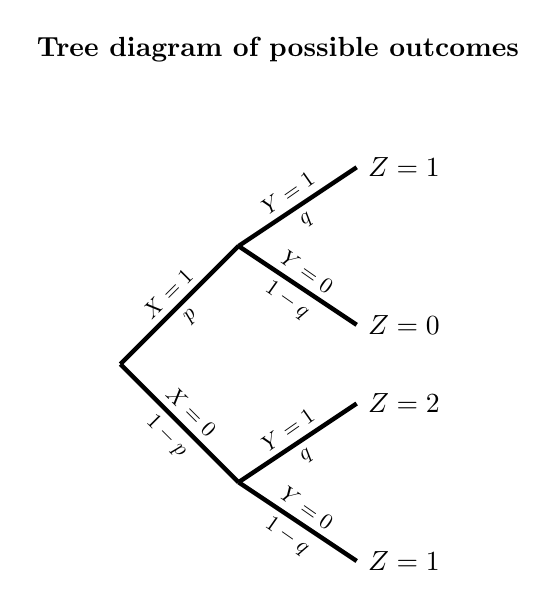
\begin{tikzpicture}
	\newcommand{\ysep}{0.5}
	\newcommand{\xsep}{0.5}
	\newcommand{\angletwo}{35}
	\newcommand{\scalethems}{0.8}
	%title
	\node  [font=\bf] at (3,4) {Tree diagram of possible outcomes};
	%first split
	\draw [ultra thick] (1,0) -- (2+\xsep,1+\ysep) 
	node [scale=\scalethems,midway, above, rotate=45] {$X = 1$}
	node [scale=\scalethems,midway, below, rotate=45] {$p$};
	\draw [ultra thick] (1,0) -- (2+\xsep,-1-\ysep) 
	node [scale=\scalethems,midway, above, rotate=-45] {$X = 0$}
	node [scale=\scalethems,midway, below, rotate=-45] {$1-p$};
	%top branches
	\draw [ultra thick] (2+\xsep,1+\ysep) -- (3+2*\xsep,2+\ysep) 
	node [scale=\scalethems,midway, above, 	rotate=\angletwo] {$Y = 1$} 
	node [scale=\scalethems,midway, below, 	rotate=\angletwo] {$q$}
	node [right] {$Z = 1$};
	\draw [ultra thick] (2+\xsep,1+\ysep) -- (3+2*\xsep,0+\ysep) 
	node [scale=\scalethems,midway, above, 	rotate=-\angletwo] {$Y = 0$}
	node [scale=\scalethems,midway, below, 	rotate=-\angletwo] {$1-q$}
	node [right] {$Z = 0$};
	%bottom branches
	\draw [ultra thick] (2+\xsep,-1-\ysep) -- (3+2*\xsep,0-\ysep) 
	node [scale=\scalethems,midway, above, 	rotate=\angletwo] {$Y = 1$}
	node [scale=\scalethems,midway, below, 	rotate=\angletwo] {$q$}
	node [right] {$Z = 2$};
	\draw [ultra thick] (2+\xsep,-1-\ysep) -- (3+2*\xsep,-2-\ysep) 
	node [scale=\scalethems,midway, above, rotate=-\angletwo] {$Y = 0$}
	node [scale=\scalethems,midway, below, rotate=-\angletwo] {$1-q$}
	node [right] {$Z = 1$};
\end{tikzpicture}
\end{center}
The above is a tree diagram; its goal is to display all of the possible combinations of $X$ and $Y$ outputs, and hence to generate all possible $Z$ outputs. Above each branch is a random variable output, and below each branch is the associated probability. The $Z$ outputs at the tips of the branches are reached by letting $Z = 1 + Y - X$. For example, the topmost $Z$ output is $Z = 1 + 1 - 1 = 1$; the $Z$ output second from the top is $Z = 1 + 0 - 1 = 0$, and so on. Notice that we defined $Z$ entirely in terms of $X$ and $Y$, so that, for example,
\[
P(Z = 0) = P(Y = 0 \;\; \textit{and} \;\; X = 1).
\]
\noindent Since we are told that $X$ and $Y$ are independent, we have (from section \ref{indep(discreterand)}),
\[
P\brac{Y = y \;\; \textit{and} \;\; X = x} = P\brac{Y = y}P\brac{X = x}, \;\;\; \text{for all possible $x, y$.}
\]
So, to find the probability of each $Z$ output, we just multiply the corresponding $X$ and $Y$ probabilities from under the branches. Hence, for example,
\[
P\brac{Y = 1 \;\; \textit{and} \;\; X = 1} = P(Y = 1)P(X = 1) = qp
\]
Notice that $Z = 1$ appears twice on the tree; this means that the set $\set{Z = 1}$ is the union of both appearances. So,
\[
P(Z = 1) = P\brac{\set{Y = 1 \;\; \textit{and} \;\; X = 1} \cup \set{Y = 0 \;\; \textit{and} \;\; X = 0}}
\]
These two events are disjoint (to see this, think about what the events are).~Hence
\begin{align*}
P(Z = 1) & = P\brac{Y = 1 \;\; \textit{and} \;\; X = 1} + P\brac{Y = 0 \;\; \textit{and} \;\; X = 0} \tag{Addition law} \\
	      & = qp + (1-q)(1-p).
\end{align*}
Finally, we can make a list of possible $Z$ values and their probabilities,
\[
P(Z = z) = \left\{
  \begin{array}{ll}
    (1-q)p, & \text{if} \; z = 0 \smallskip \\
    qp + (1-q)(1-p), & \text{if} \; z = 1 \smallskip \\
    q(1-p), & \text{if} \; z = 2 \smallskip \\
    0, & \text{otherwise}
  \end{array}
\right.
\]
As a sanity check, we should find that all of the probabilities for all the $Z$ outputs sum to 1 (as is the case with the $Y$ outputs and $X$ outputs). That is,
\begin{align*}
 (1-q)p + qp + (1-q)(1-p) + q(1-p) & = (1-q)p + qp + (1-p)(1-q+q) \\
 						    & = (1-q)p + qp + (1-p) \\
 						    & = p - qp + qp + 1 - p \\
 						    & = p + 1 - p \\
 						    & = 1.
\end{align*}

\section{The binomial distribution} \label{1 the binomial distribution} \label{binomial distribution}
We have just met the Bernoulli distribution with success parameter $p$, which was based on a discrete random variable. We will now meet our second distrbution, also based on a discrete random variable, called the binomial distribution. \\

\noindent Consider $n$ identical trials (i.e., repeated statistical experiments) where $n$ is a fixed number, and each trial idependently results in either a success or a failure. In each trial the probability of success is the same value, $p$. \\

\noindent \textit{For example, we could be tossing a fair coin four times. If success is tossing a head, then $n = 4$ and $p = \frac{1}{2}$.} \\

\noindent Let $X$ count the total number of successes. Since we have $n$ trials, we can have up to $n$ successes. So, $X$ is a random variable whose outputs belong to the set $\set{0,1,\ldots,n}.$ \\

\noindent  Suppose that $X = k$ for some value $k$ in the set of possible outputs of $X$. This means that after $n$ trials we have had $k$ successes. Each of the $k$ successes has probability $p$, and the remaining $n-k$ trials are failures, which occur with probability $1-p$. The trials are independendent, so their probabilities can be multiplied. Hence, a pattern of $k$ successes with $n - k$ trials must have probability
\[
p^k(1-p)^{n-k}
\]

\noindent However, there may be more than one way that the $k$ successes can occur; for example, if we are flipping a coin 4 times and we get 2 heads, we might get heads on the first two flips, or the last two flips, or some other pattern. How many ways can the $k$ successes occur in the $n$ trials? We need to use combinatorics. Specifically, we need to use the binomial coefficients from section \ref{sec313} (you are encouraged to read this section for a refresher). Choosing $k$ successes from $n$ trials is a case of unordered sampling without replacement (i.e., we dont care which order the successes happened in, in fact the order of the trials is fixed, we only care which trials were a success). Hence, the number of ways that the $k$ successes can occur is
\[
\binom{n}{k}.
\]
Thus, to find the probability of the $k$ successes, we need to take the probability of success from one pattern, $p^k(1-p)^{n-k}$, then multiply it by the number of possible patterns, $\binom{n}{k}$. Now we have everything we need to define a function rule, $p(k)$, which returns the probability of the $k$ successes, \label{binom pmf}

  	\bigskip
	
	\hfil\fbox{
	\begin{minipage}{0.45\columnwidth}{
	
	\vskip 0.1cm
	\begin{center}
	$\displaystyle{P(X = k) = p(k) = \binom{n}{k}p^k(1-p)^{n-k}}$
	\end{center}
	}
	\end{minipage}}
	\bigskip
	\bigskip

\noindent This is the pmf of the binomial distribution (the name comes from its relationship to the binomial coefficients). The binomial distribution is used so often that we use the abbreviation \textbf{Bin($\boldsymbol{n,p}$)}, short for Binomial($n,p$), which is the \textbf{binomial distribution with parameters $\boldsymbol{n}$ and $\boldsymbol{p}$}. To indicate that the discrete random variable, $X$, is distributed according to the binomial disribution, we write \label{Bin(n,p)}

  	\bigskip
	
	\hfil\fbox{
	\begin{minipage}{0.3\columnwidth}{
	
	\vskip 0.1cm
	\begin{center}
	$X \sim$ Bin($n,p$)
	\end{center}
	}
	\end{minipage}}
	\bigskip
	\bigskip

\noindent For better intuition, we can visualise it using our 4 coin flips example ($n = 4$ trials), with $k = 2$ successes: \\
\textit{Tails were left blank to simplify the diagram}
\begin{center}
\begin{tikzpicture}
\newcommand{\circsizes}{0.3}
\draw [thick,fill = white] (0,0) circle (\circsizes cm);
\draw [thick,fill = white] (1,0) circle (\circsizes cm) node {H};
\draw [thick,fill = white] (2,0) circle (\circsizes cm) node {H};
\draw [thick,fill = white] (3,0) circle (\circsizes cm);

\draw (0-\circsizes,0.5) -- (3+\circsizes,0.5);

\draw [thick,fill = white] (0,1) circle (\circsizes cm);
\draw [thick,fill = white] (1,1) circle (\circsizes cm) node {H};
\draw [thick,fill = white] (2,1) circle (\circsizes cm);
\draw [thick,fill = white] (3,1) circle (\circsizes cm) node {H};

\draw (0-\circsizes,1.5) -- (3+\circsizes,1.5);

\draw [thick,fill = white] (0,2) circle (\circsizes cm) node {H};
\draw [thick,fill = white] (1,2) circle (\circsizes cm);
\draw [thick,fill = white] (2,2) circle (\circsizes cm) node {H};
\draw [thick,fill = white] (3,2) circle (\circsizes cm);

\draw (0-\circsizes,2.5) -- (3+\circsizes,2.5);

\draw [thick,fill = white] (0,3) circle (\circsizes cm);
\draw [thick,fill = white] (1,3) circle (\circsizes cm);
\draw [thick,fill = white] (2,3) circle (\circsizes cm) node {H};
\draw [thick,fill = white] (3,3) circle (\circsizes cm) node {H};

\draw (0-\circsizes,3.5) -- (3+\circsizes,3.5);

\draw [thick,fill = white] (0,4) circle (\circsizes cm);
\draw [thick,fill = white] (1,4) circle (\circsizes cm)node {H};
\draw [thick,fill = white] (2,4) circle (\circsizes cm)node {H};
\draw [thick,fill = white] (3,4) circle (\circsizes cm);

\draw (0-\circsizes,4.5) -- (3+\circsizes,4.5);

\draw [thick,fill = white] (0,5) circle (\circsizes cm)node {H};
\draw [thick,fill = white] (1,5) circle (\circsizes cm)node {H};
\draw [thick,fill = white] (2,5) circle (\circsizes cm);
\draw [thick,fill = white] (3,5) circle (\circsizes cm);

\draw [dashed] (0-2*\circsizes,5.7) -- (3+2*\circsizes,5.7)node [above,midway] {$n = 4$ trials};
\draw [dashed] (3+3*\circsizes,0-2*\circsizes) -- (3+3*\circsizes,5.5) node [above,midway, rotate=-90] {$\binom{n}{k} = \binom{4}{2} = 6$ possible patterns};
\end{tikzpicture}
\end{center}
For a fair coin, $p = \frac{1}{2}$, so the probability of success for each pattern is
\[
p^k(1-p)^{n-k} = \bfrac{1}{2}^2\brac{1-\frac{1}{2}}^{4-2} = \bfrac{1}{2}^4 = \frac{1}{16}.
\]
There are $\binom{n}{k} = 6$ possible disjoint patterns so the probability of their union is the sum of their probabilities, i.e., we have 6 times the probability of success from 1 pattern, i.e., 
\[
\binom{n}{k}p^k(1-p)^{n-k} = 6 \times \frac{1}{16} = \frac{3}{8}
\]
Since we have a formula for $p(k)$, we could have done all of this in one single step: 
\[
P(X = 2) = p(2) = \binom{4}{2}\bfrac{1}{2}^2\brac{1-\frac{1}{2}}^{4-2} = 6 \times \frac{1}{16} = \frac{3}{8}.
\]

\subsection{Checking validity of Bin($\boldsymbol{n,p}$)} \label{validity of bin}
Since we now have a function rule for the pmf of the binomial distribution, it is good practice to check that this rule satisfies the probability measure axioms (the axioms are in section \ref{paxioms}). \\

\noindent Let $X \sim$ Bin($n,p$) so that $p(k) = \binom{n}{k}p^k(1-p)^{n-k}$. Now, \\

\noindent \textbf{Axiom 2} is the easiest to check; we require that $P(A) \geq 0$ for any event $A \subseteq \Omega$. In other words, we have to check that,
\[
P(X = k) = p(k) \;\;\; \text{is always non-negative.}
\]
Now, $\binom{n}{k}$ is always non-negative. Also, $p^k$ is always non-negative since $p \in [0,1]$. Furthermore,
\[
0 \leq p \leq 1 \qquad \text{implies} \qquad 0 \geq -p \geq -1 \qquad \text{implies} \qquad 1 \geq 1 - p \geq 0.
\]
So $(1-p)$ is always greater than zero; hence $(1-p)^{n-k}$ is always positive. So, it follows that $p(k)$ is a product of three positive terms, and hence its output is always positive. Thus axiom 2 is satisfied. \\

\noindent \textbf{Axiom 3} is not something that we need to check for distributions; it is more perscriptive. Since $\set{X = k_1}$ is disjoint from $\set{X = k_2}$ whenever $k_1 \neq k_2$ (see section \ref{disjran}), axiom 3 tells us that,
\[
P(\set{X = k_1} \; \cup \; \set{X = k_2}) = P(X = k_1) + P(X = k_2) = p(k_1) + p(k_2).
\]
Which can be extended to unions of arbitrarily many events, $\set{X = k_i}$. So, of particular interest to us when we want to find a cumulative distribution function, we can write
\[
P(X \leq n) = \sum_{k \leq n} P(X = k).
\]
The subscript ``$k \leq n$'' under the summation symbol means that we sum over all of the $k$ that are less than or equal to $n$. \\

\noindent \textbf{Axiom 1} is the most fun to check; we require that $P(\Omega) = 1$. Since $X$ counts possible successes, the domain of $X$ is $\set{0,1,\ldots,n}$. So we require
\[
P(\set{X = 0} \cup \set{X = 1} \cup \ldots \cup \set{X = n}) = 1
\]
Using axiom 3 (or the addition law), this means we require that
\[
p(0) + p(1) + \ldots + p(n) = 1.
\]
In summation notation this is
\[
\sum_{k=0}^n p(k) = \sum_{k=0}^n \binom{n}{k}p^k(1-p)^{n-k} = 1.
\]
To check this, we need to use the \textbf{binomial theorem} from section \ref{secbinom} in lecture \ref{lect3}. The binomial theorem states that
\[
(x+y)^n = \sum_{k=0}^n \binom{n}{k}x^ky^{n-k}
\]
If we make the substitution $x = p$ and $y = (1-p)$ then we get,
\[
(p + (1-p))^n = \sum_{k=0}^n \binom{n}{k}p^k(1-p)^{n-k}
\]
On the left hand side we have $p + (1-p) = p - p + 1 = 1$. So,
\[
1 = \sum_{k=0}^n \binom{n}{k}p^k(1-p)^{n-k}.
\]
But the right hand side is exactly our expression for $\displaystyle{\sum_{k=0}^n p(k)}$. Hence
\[
\sum_{k=0}^n p(k) = 1, \qquad \text{as required.}
\]
So axiom 1 is satisfied.
%Since we have just expressed $Z$ in terms of $X$ and $Y$, we can conclude that $Z$ is \textit{dependent} on $X$ and $Y$ (we will not use this to find the probabilities for $Z$, but). 


\subsection{Example}
Calculate $P(X = k)$ for $k = 3$, for the example of tossing an \textbf{unfair} coin 5 times, where success is tossing a head. Since the coin is unfair, let $p = \frac{1}{4}$. \\

\noindent \textit{Solution:} \\
Let $X$ be the discrete random variable that counts the number of successes (i.e., the number of heads) after 5 tosses. This is a situation with 5 identical trials, each independently resulting in success or failure, and we are counting the number of successes, so $X \sim$ Bin($n,p$) with $n = 5$, and $p = \frac{1}{4}$; i.e., $X \sim$ Bin($5,\frac{1}{4}$). Therefore,
\[
P(X = k) = \binom{5}{k}\bfrac{1}{4}^k\brac{1 - \frac{1}{4}}^{5-k}.
\]
So,
\begin{align*}
P(X = 3) & = \binom{5}{3}\bfrac{1}{4}^3\brac{\frac{3}{4}}^{5-3} \\
	      & = \frac{5!}{3!2!} \frac{1}{4^3}\bfrac{3^2}{4^2} \tag{using index laws} \\
	      & = \frac{5\times 4}{2} \frac{3^2}{4^{3+2}} \tag{using index laws} \\
	      & = 10\frac{3^2}{4^5} \\
	      & \approx 0.088. 
\end{align*}

\subsection{Example} \label{ex10.2.2}
Suppose that a factory run of $5000$ electrical fuses contains $5\%$ defectives. If a sample of $7$ fuses is tested, find the probability of observing \textbf{at least one} defective fuse. \\

\noindent \textit{Solution:} \\
Let $X$ be the discrete random variable that counts the number of defective fuses in the $7$ fuse sample. We can view the $7$ fuse sample as $7$ identical independent trials, each with some fixed probability $p$ of success (\textit{where success is the fuse being defective}). Hence $X \sim $ Bin($7,p$). Since $5\%$ of the fuses are defective, we know that $p = \frac{5}{100} = 0.05$. When asked to find the probability that at least one fuse is defective, we should translate this as asking for the probability $P(X \geq 1)$. Therefore
\begin{align*}
P(X \geq 1) & = 1 - P(X = 0) \tag{since $P(\Omega) = 1$, and $X \geq 0$} \\
		  & = 1 - \binom{7}{0}\brac{0.05}^0\brac{0.95}^7 \\
		  & = 1 - \frac{7!}{7!0!}\brac{0.95}^7 \\
		  & = 1 - 0.95^7
		  & \approx 0.3.
\end{align*}
We did make one simplifying assumption which, though not entirely accurate, should not have affected our final answer significantly. Can you see what this assumption was? \\

\noindent We assumed that the $7$ fuse sample was a case of $7$ identical (independent) trials. This is not entirely true because each time we select a fuse we reduce the size of the pool (which has size 5000) by 1. This means that if one fuse is found to be defective (or functional), then the probability of the next fuse being defective (or functional) is slightly altered. However, the sample size (7) is very small in comparison to the size of the pool (5000). So, this assumption will have a negligable impact.  



\subsection{Example}
Below is a plot of the pmf of the binomial distribution with $n = 5$ and $p = \frac{1}{2}$:
\begin{center}
\begin{tikzpicture}[yscale=0.7,xscale=1.2]
\draw [->,gray] (0,-0.1) -- (0,11) node [above left] {$p(k)$};
\draw [->,gray] (-0.1,0) -- (6,0) node [below right] {$k$};
\foreach \x in {1,2,3,4,5}{
\draw (\x,0) node {$|$} node [below = 2mm] {$\x$};
}
\foreach \y in {1,2,3,4,5,6,7,8,9,10}{
\draw (0.1,\y) -- (-0.1,\y) node [left] {$\frac{\y}{32}$};
}
\draw [fill = black] (0,1) ellipse (0.07cm and 0.1cm);
\draw [fill = black] (5,1) ellipse (0.07cm and 0.1cm);

\draw [fill = black] (1,5) ellipse (0.07cm and 0.1cm);
\draw [fill = black] (4,5) ellipse (0.07cm and 0.1cm);

\draw [fill = black] (2,10) ellipse (0.07cm and 0.1cm);
\draw [fill = black] (3,10) ellipse (0.07cm and 0.1cm);
\end{tikzpicture}
\end{center}

Below is a plot of the cdf of the binomial distribution with $n = 5$ and $p = \frac{1}{2}$:
\begin{center}
\begin{tikzpicture}[yscale=0.23,xscale=1.2]
\draw [->,gray] (0,-0.6) -- (0,34) node [above left] {$p(k)$};
\draw [->,gray] (-0.7,0) -- (6,0) node [below right] {$k$};
\foreach \x in {1,2,3,4,5}{
\draw (\x,0) node {$|$} node [below = 2mm] {$\x$};
}
\foreach \y in {10,20,30}{
\draw (0.1,\y) -- (-0.1,\y) node [left] {$\frac{\y}{32}$};
}
\draw (0.1,32) -- (-0.1,32) node [left] {$1$};
%\draw [fill = black] (0,1) ellipse (0.07cm and 0.3cm);
%\draw [fill = black] (5,1) ellipse (0.07cm and 0.1cm);
%
%%\draw [fill = black] (1,5) ellipse (0.07cm and 0.1cm);
%%\draw [fill = black] (4,5) ellipse (0.07cm and 0.1cm);
%%
%%\draw [fill = black] (2,10) ellipse (0.07cm and 0.1cm);
%%\draw [fill = black] (3,10) ellipse (0.07cm and 0.1cm);

\draw [dashed] (0,32) -- (5,32);

\newcommand{\cdfcoordAi}{(0,1)}
\newcommand{\cdfcoordAf}{(1,1)}

\newcommand{\cdfcoordBi}{(1,1+5)}
\newcommand{\cdfcoordBf}{(1+1,1+5)}

\newcommand{\cdfcoordCi}{(2,1+5+10)}
\newcommand{\cdfcoordCf}{(2+1,1+5+10)}

\newcommand{\cdfcoordDi}{(3,1+5+10+10)}
\newcommand{\cdfcoordDf}{(3+1,1+5+10+10)}

\newcommand{\cdfcoordEi}{(4,1+5+10+10+5)}
\newcommand{\cdfcoordEf}{(4+1,1+5+10+10+5)}

\newcommand{\cdfcoordFi}{(5,1+5+10+10+5+1)}
\newcommand{\cdfcoordFf}{(5+1,1+5+10+10+5+1)}

\draw [dashed] \cdfcoordAf -- \cdfcoordBi;
\draw [dashed] \cdfcoordBf -- \cdfcoordCi;
\draw [dashed] \cdfcoordCf -- \cdfcoordDi;
\draw [dashed] \cdfcoordDf -- \cdfcoordEi;
\draw [dashed] \cdfcoordEf -- \cdfcoordFi;

\draw [ultra thick] (-0.7,0) -- (0,0);
\draw [fill = white, thick] (0,0) ellipse (0.07cm and 0.3cm);

\draw [fill = black] \cdfcoordAi ellipse (0.07cm and 0.3cm);
\draw [ultra thick] \cdfcoordAi -- \cdfcoordAf;
\draw [fill = white] \cdfcoordAf ellipse (0.07cm and 0.3cm);

\draw [fill = black] \cdfcoordBi ellipse (0.07cm and 0.3cm);
\draw [ultra thick] \cdfcoordBi -- \cdfcoordBf;
\draw [fill = white] \cdfcoordBf ellipse (0.07cm and 0.3cm);

\draw [fill = black] \cdfcoordCi ellipse (0.07cm and 0.3cm);
\draw [ultra thick] \cdfcoordCi -- \cdfcoordCf;
\draw [fill = white] \cdfcoordCf ellipse (0.07cm and 0.3cm);

\draw [fill = black] \cdfcoordDi ellipse (0.07cm and 0.3cm);
\draw [ultra thick] \cdfcoordDi -- \cdfcoordDf;
\draw [fill = white] \cdfcoordDf ellipse (0.07cm and 0.3cm);

\draw [fill = black] \cdfcoordEi ellipse (0.07cm and 0.3cm);
\draw [ultra thick] \cdfcoordEi -- \cdfcoordEf;
\draw [fill = white] \cdfcoordEf ellipse (0.07cm and 0.3cm);

\draw [fill = black] \cdfcoordFi ellipse (0.07cm and 0.3cm);
\draw [ultra thick] \cdfcoordFi -- \cdfcoordFf;
\end{tikzpicture}
\end{center}







\section{Our usage of $\boldsymbol{p}$, $\boldsymbol{p(k)}$, $\boldsymbol{P(X = k)}$ and $\boldsymbol{F(k)}$} \label{pp(k)P(X=k)f(k)F(K)}
Up to this point we have introduced three different notations involving the letter $p$. To avoid confusion we will briefly clarify, again, what each of these notations represents. \\

\noindent \textbf{$\boldsymbol{p}$} is a number between $0$ and $1$. It represents a probability. For example $p = \frac{1}{2}$ is the probability of getting heads when flipping a fair coin. \\

\noindent \textbf{$\boldsymbol{p(k)}$} represents a function rule. This is just like writing $g(x)$ or $h(x)$ or any other choice of letter to label a function. However, we will use $p(x)$ specifically when we are referring to the probability mass function (pmf) associated with a discrete random variable. For example, if $X \sim $ Bin($n,p$) then the pmf associated with $X$ is
\[
p(k) = \binom{n}{k}x^ky^{n-k}
\]
Soon, when we look at continuous random variables in more detail, we will begin using the symbol $f(x)$ to refer specifically to the \textit{probability density function} (pdf) of a continuous random variable. We have not yet introduced probability density functions. \\

\noindent \textbf{P(X = k)} is interpreted as ``the probability of the event $\set{X = k}$.'' This is also a function, and often we have $P(X = k) = p(k)$. However, $P(X = k)$ is more general than $p(k)$, which is just a particular function rule. \\

\noindent \textbf{F(k)} is also a function; it represents the cumulative distribution function (cdf) of any random variable (discrete of continuous).


















